\section{模型}
我们的DIP由两方面构成。一方面在于构建一个优秀的排名系统。其意义在于能为用户提供一个良好的推荐环境。正如我们在App Store上见到的,好的App在排行榜上拥有更显著的位置进而能受到更多用户的关注。而用户能通过排行榜上直接获取高质量的App无疑能提高其体验。同时,App的排名也可以用到关键词搜索中,正如google,baidu等搜索引擎以及淘宝,京东等电商平台中的搜索功能一样,与关键词相关的app将按排名分顺序展示在搜索结果中,增加用户对此次搜索结果的满意程度。

DIP另一方面,正如我们在第二章所提到的,在于为排名高的开发提供额外的奖励,如同实际中的各种评奖活动。这进一步增加了开发者设计优秀DApp的动机,对整个生态的开发起到了促进作用。

NR值是我们衡量用户价值的重要依据。然而NR的更新是一天一次,远远小于DIP发放奖励的间隔时间。我们的做法是将一次评选过程分成阶段,根据所有用户NR变化的数据(cite),然后取整数$t$使得绝大部分用户的NR值在$t$天的变化幅度小于某个阈值$\tau$。我们把连续$t$天作为一个阶段,通过取这一阶段类用户的平均NR值以及调用DApp数据来计算用户的排名分及最终奖励,并把一个评选周期内所有阶段的数据取其平均值最为最终结果。下面介绍在一个阶段内我们的模型运作。


{\color{red} 发奖励时间,加个NR变化图}

\subsection{字母表示}
\begin{itemize}
	\item $\mathcal{A}=\{a_1,a_2,...,a_m\}$表示所有参与此阶段评选的用户的集合。只要用户在此阶段中调用过任何DApp则可认为他参与了评选。
	\item $\mathcal{D}=\{d_1,...,d_n\}$表示此阶段所有DApp的集合。
	\item $e_{ij},i=1,2,...,m, j=1,2,...,n$表示用户$a_i$对DApp $d_j$的调用次数。因我们的系统是基于区块链的,具第一章所提到的公开性,去中心化等特性,我们的模型和传统app store上的评分系统有所不同。具体而言,我们缺少一个中心化系统用于实现用户给DApp评分的功能。同时,因为用户每次调用DApp都是访问合约地址,所以也不存在App Store里的下载量的统计。在我们的模型中,调用次数是唯一能获取且之后会用到的初始数据。虽然用户在调用过程中产生的资金交互和gas费用也可以被统计到,但根据第二章的说明这些将不会被考虑进去。用户和DApp之间的交互可以用图\ref{fig:interact}中的这个二分图来表示。
	\item $NR_i, i=1,2,...,m$表示参与评选的用户在此阶段的平均NR值。\cite{Nabulasyellowpaper}中已经证明NR值是衡量一个用户的有效价值尺度,故我们也把其用作DIP模型中用于决定用户投票权重的重要指标。
	\item $NR_{ij}, i=1,2,...,m,j=1,2,...,n$表示用户$a_i$对DApp $d_j$的分贡献值。可以理解为$a_i$愿意为$d_j$投的票数。在我们的模型里有$a_i$对所有DApp的调用次数决定。
	\item $scoer_j, j=1,2,...,n$,表示DApp $d_j$的排名分,由该DApp从用户获得的所有分贡献值决定。同时,排名分的高低直接决定了DApp在排行榜上所处的位置。一种对排名分最简单的定义方式为所有分贡献值相加。而我们的模型采取了更合理的排名分计算方式。
	\item $M$表示星云团队用于给与开发者奖励的最大值。实际发放的奖励总额会根据该阶段社区参与度来适当进行衰减。
	\item $u_j, j=1,2,...,n$,表示DAPP $d_j$开发者最终获得的奖励,这个奖励由奖励总额以及所有$Dapp$的排名分共同决定。生活中常见的评奖方式通常具有凹函数性质,例如第一名10000元,第二名5000元,第三名2000元。我们的奖励函数具有同样性质且具有更高的可扩展性。
\end{itemize}
	 \begin{figure}
	 	\centering
	 	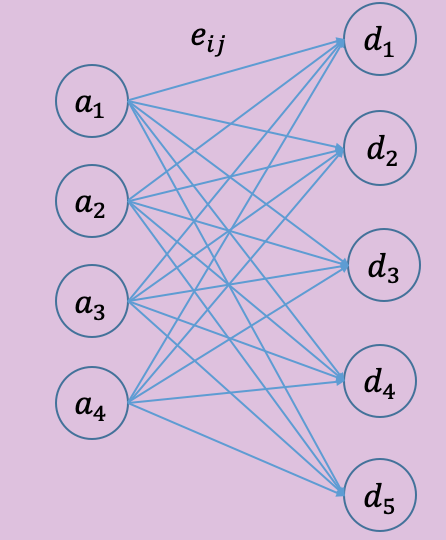
\includegraphics[width = 0.4\textwidth]{../common/m2.png}
	 	\caption{用户与DApp间的交互 \label{fig:interact}}
	 \end{figure}
\subsection{行为介绍}
在我们的模型中,一个用户$a_i \in \mathcal{A}$本质上是一个账户地址,正如黄皮书所提到的,一个用户可以控制多个账户地址。由于建立新的账户地址是没有成本的,用户可以伪造出多个受他控制的地址进行投票,进行所谓女巫攻击。但受NR定义中的财产中值等限制这些伪造的账户NR值都很低。同时,一个DApp也对应于一个合约地址。DApp开发者可以选择将自己的Dapp分成多个地址,相当将一个DApp拆分成多个低质量的DApp,并且获得这些DApp的总奖励。

一个DApp开发者也可以线下收买用户为他进行投票,正如各种选举拉票一样,这种行为本质上无法制止,但我们可以通过机制设计加大收买所需要付出的代价。